\documentclass[acmtog, screen]{acmart}

\usepackage[utf8]{inputenc}
\usepackage[spanish]{babel}
\usepackage{graphicx}
\graphicspath{{../fig/}}

\usepackage{booktabs} % For formal tables
\usepackage{hyperref}
\usepackage{amsmath}

% Document starts
\begin{document}
% Title portion
\title{Desarrollo de Sistemas Inteligentes - Trabajo final}

\author{Luis Cabañero Gómez}
\email{Luis.Cabanero@alu.uclm.es}

\maketitle

Enlace a repositorio GitHub: \url{https://github.com/Xiul109/DSI}

Enlace a vídeo de Youtube: \url{https://www.youtube.com/watch?v=iElI5cadc2k&feature=youtu.be}

\section{Introducción}
Esta memoria describe el proceso que se ha seguido para llevar a cabo el trabajo final de la asignatura. Este consiste en utilizar los datos de la \href{https://pslcdatashop.web.cmu.edu/KDDCup/}{KDDCup 2010} para resolver el problema propuesto o para proponer un nuevo problema y resolverlo. En este caso se ha optado por la segunda opción.

\subsection{Toma de contacto con los datos}
Los datos describen el log generado por un tutor inteligente de álgebra es un interacción con un alumno, representando cada una de las filas un paso que sigue el alumno para resolver un problema específico. Cada una de estas filas almacena la siguiente información relacionada con cada paso:
\begin{itemize}
	\item \textbf{Nombres e identificadores}: Cada paso se identifica unívocamente mediante la combinación: nombre de alumno, nombre del problema, nombre de la unidad en la que se encuentra, veces que el alumno ha visto ese problema y nombre del paso. De estos identificadores, los cuatro primeros sirven para identificar un problema específico que es resuelto por un alumno. Un mismo problema puede aparecer en dos o más unidades diferentes. Un alumno puede resolver más de una vez el mismo problema (aunque cambian los números).
	\item \textbf{Marcas de tiempo}: Hay una marca de tiempo para el inicio del paso, el fin del paso, la primera transacción del paso y la transacción en la que se introduce la respuesta correcta. Un factor a tener en cuenta en relación a las marcas de tiempo es que un paso puede empezar sin que el anterior haya terminado, pero esto no debe interpretarse como ruido, sino como una característica del tutor inteligente.
	\item \textbf{Duraciones}: Hay tres campos que representan duraciones: la duración del paso, la duración del paso si este ha sido correcto en el primer intento y la duración del paso si este ha sido incorrecto en el primer intento. De estos campos, los dos últimos contienen información redundante, ya que la duración que muestran es la misma y si el paso se completó correctamente al primer intento lo refleja otro campo.
	\item \textbf{Transacciones correctas, incorrectas y pistas}: Por cada paso se registran cuantos resultados correctos se han introducido, cuantos incorrectos y cuantas pistas se han solicitado. Se pueden registrar más de un resultado correcto porque el formulario no siempre se cierra a la hora de introducir un valor y cada vez que se actualiza el valor se registra como correcto, por lo que su valor no es muy relevante.
	\item \textbf{Correct First Attempt}: Este campo muestra un 0 si el paso no se ha resuelto en el primer intento o si se han usado pistas y un 1 si se ha resuelto correctamente en el primer intento y sin pistas. A priori podría pensarse que este campo sólo puede valer uno cuando el número de valores incorrectos y pistas vale 0, sin embargo también se ve afectado por la casuística descrita en el punto anterior.
	\item \textbf{Knowledge Components (KC)}: Este campo se representa como una cadena de texto y se refiere a los conocimientos necesarios para resolver un paso concreto.
	\item \textbf{Opportunity:} Este campo representa un contador asociado a un KC específico que se incrementa en uno cada vez que un alumno se encuentra con ese KC.
\end{itemize}

\subsection{Exposición del problema}
El problema propuesto consiste en predecir si un determinado problema le resultará de una dificultad fácil, difícil o moderada a un alumno. Para poder establecer si un problema es más o menos fácil, se tienen en cuenta el número de pistas que pide y el número de respuestas incorrectas dadas en total en el problema. Los pasos generales que se han seguido para la resolución de este problema específico han sido:
\begin{enumerate}
	\item Agrupar los pasos en problemas e identificar la dificultad del problema en función de las pistas y el número de respuestas incorrectas.
	\item Crear esquemas generales para definir los problemas, especialmente de cara a obtener los KC necesarios para resolver un tipo de problema específico.
	\item Preparar los datos del modelo teniendo en cuenta la dimensión temporal de los datos.
	\item Definir el modelo.
	\item Entrenar y evaluar el modelo.
\end{enumerate}
Merece la pena mencionar que todas las pruebas se han realizado únicamente sobre el archivo ``algebra\_2005\_2006\_train.txt'', sin embargo, al tener todos la misma estructura, el programa puede trabajar con otros archivos.

\subsection{Herramientas utilizadas}
Todo el proceso para la resolución del problema ha sido implementado en el lenguaje de programación Python y haciendo uso de las siguientes librerías:
\begin{itemize}
	\item \textbf{pandas}: Esta librería se utiliza para cargar los ficheros csv y para poder acceder a sus estructuras de datos, que permiten trabajar de una manera cómoda y eficiente.
	\item \textbf{NumPy}: Esta librería aporta estructuras de datos eficientes y funciones para operar sobre esas estructuras de datos.
	\item \textbf{scikit-learn}: Esta librería se utiliza para clasificación, para clustering y para validación.
	\item \textbf{matplotlib}: Ha sido utilizada para graficar puntos coloreados representando los grupos de dificultad identificados.
	\item \textbf{seaborn}: Esta librería se ha utilizado para graficar una matriz de confusión.
\end{itemize}

\section{Preprocesamiento}
Esta es la fase en la que más esfuerzos y tiempo se ha dedicado, ya que abarca todas las transformaciones de datos que han sido necesarias para entrenar el modelo.
\subsection{Cargado de datos}
Al cargar los datos, se han realizado diversas transformaciones para poder trabajar mejor con los mismos.

Lo primero que se ha hecho ha sido incorporar un mecanismo para poder cargar solo un subconjunto de los datos, de tal manera que la ejecución completa tardará menos tiempo. Este subconjunto se ha elegido de manera aleatoria en función de un porcentaje que se puede regular y se selecciona en función de los alumnos, es decir, que si el porcentaje establecido es del 10\%, entonces se seleccionan los datos en los que aparecen el 10\% de los alumnos.

A continuación se han transformado algunas columnas, como las correspondientes a las fechas, las cuales estaban representadas como cadenas de texto y se han convertido al tipo pandas.DateTime, que permite realizar operaciones entre fechas. Las columnas KC y Opportunity representaban mediante cadenas de texto listas de elementos separando cada uno mediante la cadena ``$\sim\sim$'' y se han transformado en listas (en el caso de KC de cadenas de texto y en el caso de Opportunity de enteros) y se han cambiado los valores vacíos por listas vacías.

\subsection{Agrupamiento de datos}
\subsubsection{Agrupando pasos en problemas}
Ya que los datos representan pasos para resolver un problema y en el nuevo planteamiento propuesto se quiere trabajar con problemas en lugar de con pasos, es necesario agrupar los pasos. A la hora de realizar esta agrupación es relevante considerar que campos se van a usar y cómo se van a combinar:
\begin{itemize}
	\item Para los \textbf{aciertos, fallos y pistas} se han sumado la cantidad de cada uno en cada paso.
	\item Para \textbf{Correct First Attempt} se ha calculado la media de todos los pasos, de tal manera que el valor representa el porcentaje de pasos del problema que se han resuelto a la primera.
	\item El \textbf{tiempo de inicio} se ha definido como el menor de los tiempos de inicio de los pasos y el \textbf{tiempo de fin} como el mayor de los tiempos de fin de los pasos.
	\item La \textbf{duración de los pasos} se ha sumado para obtener una duración total del problema, sin embargo, también se ha creado un campo nuevo de duración que se define como el tiempo de fin menos el tiempo de inicio. Esto se ha hecho porque la suma de la duración de los pasos no siempre es igual a la duración del problema, ya que es posible estar realizando simultáneamente dos o más pasos. Como el nuevo campo de duración tiene valores nulos, debido a que algunas fechas faltan, estos han sido sustituidos por el valor de la suma de duraciones de los pasos.
	\item Los \textbf{KC} se han combinado en varias etapas: primero se han concatenado todas las listas de cada paso. Después se ha creado una nueva columna por cada KC diferente (alrededor de 100, aunque varía en función del subconjunto de datos elegidos al cargar el fichero) y se inicializan todos los valores a 0. A continuación en cada problema se pone un 1 en la columna relativa a un KC específico si aparece al menos una vez ese KC en la lista que concatena los KC de los pasos. Esto acaba generando una matriz dispersa.
\end{itemize}
Algunos estos campos se han renombrado para luego trabajar más cómodamente con ellos y para que tengan más sentido en el contexto de los problemas. En el caso del campo opportunity, se ha omitido, ya que aporta información redundante que ya proporcionan los KC.

\begin{figure*}[ht]
	\centering
	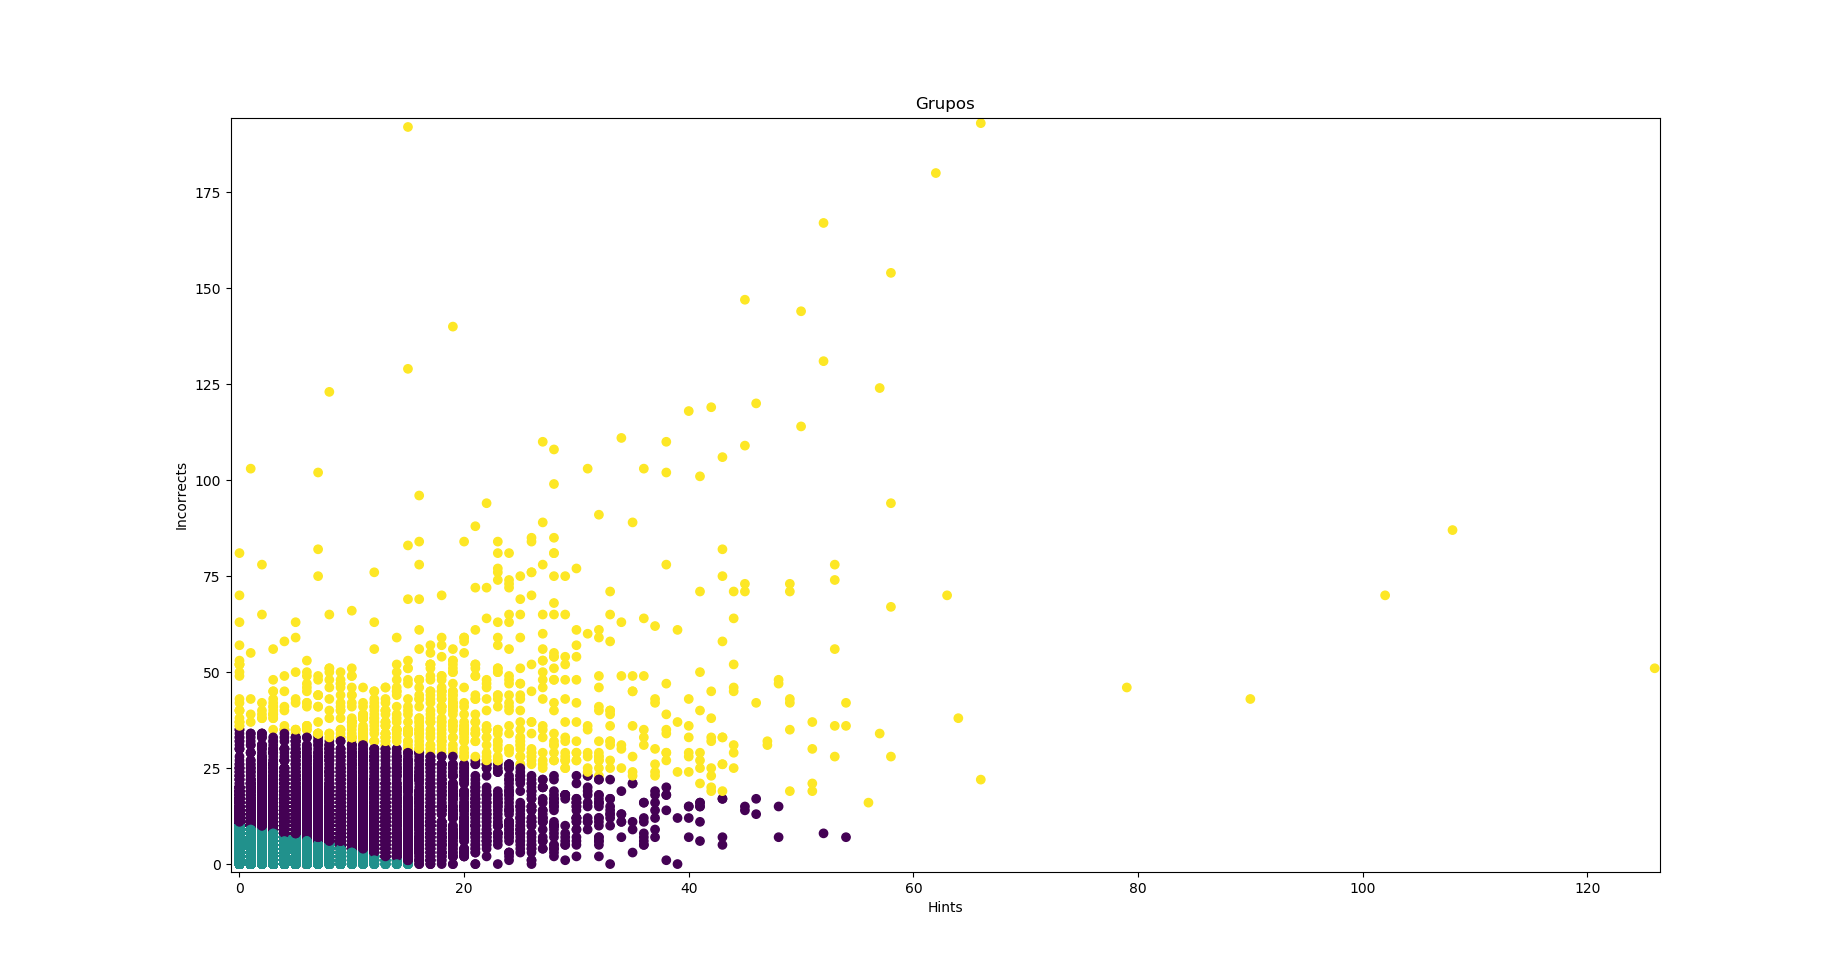
\includegraphics[width=0.95\textwidth]{grupos}
	\caption{Representación de la agrupación de los problemas mediante KMeans en función de las pistas y las respuestas incorrectas.}
	\label{fig:grupos}
\end{figure*}

Lo último que se hace para agrupar los problemas es determinar el nivel de dificultad de cada uno en función de las pistas y el número de respuestas incorrectas. Para ello se ha utilizado el algoritmo de clustering KMeans y se han especificado que sean 3 grupos. El resultado del clustering se puede apreciar en la figura \ref{fig:grupos}. Aunque la cantidad de elementos de los grupos puede parecer bastante equilibrada a priori, en realidad es bastante dispersa, teniendo el grupo que corresponde a los problemas más fáciles bastantes más elementos que el que corresponde a los problemas intermedios que, a su vez, tiene bastantes más elementos que los problemas difíciles.

El algoritmo KMeans identifica cada grupo con una etiqueta numérica, en este caso serían 0,1 y 2. En cada ejecución la etiqueta numérica asociada a cada grupo puede cambiar, por lo que no se puede decir de manera absoluta que una etiqueta numérica corresponde siempre a la misma dificultad. Para poder determinar la dificultad asociada a cada etiqueta, se ha definido una función que asocia el grupo con una media de pistas más baja a la dificultad fácil, el que tiene un número de pistas media más alta a la dificultad difícil y el restante a la dificultad moderada. 

\subsubsection{Agrupando problemas en esquemas generales}
Se ha querido agrupar todas las veces que aparece un problema principalmente para poder determinar que KCs suele requerir. Debido a que muchos problemas pueden mostrar pasos opcionales, es fácil que un problema se resuelva usando diferentes KC en dos momentos diferentes. Para poder determinar qué importancia tiene cada KC en cada problema, se han promediado los KC a la hora de agrupar, de tal manera que el nuevo valor representa la importancia de un KC concreto a la hora de resolver un problema, significando un 1 que ese KC es imprescindible y un 0 que es irrelevante. Al hacer esta agrupación es posible obtener una referencia general de un problema. Para el problema que se pretende resolver lo idóneo sería tener una definición específica del problema y no tener que inferirla a partir de los datos.

\subsection{Preparación de datos del modelo}
Una vez ya generados los datos de los problemas y de los esquemas de problemas se puede empezar a preparar los datos que se utilizarán para entrenar el modelo. La idea de estos datos es que cada fila represente el encuentro entre un problema y un alumno, definiéndose este por el conocimiento e historial que ha tenido al realizar previamente otros problemas, con lo que se consideraría el carácter temporal de los datos.

Para representar los conocimientos de los alumnos se ha creado una columna nueva por cada KC que representa el nivel de capacidad que tiene el alumno con ese KC. En cuanto al historial del alumno, se han creado columnas que almacenan el número de problemas que ha hecho previamente, la media de pistas por problema previo, la media de fallos por problema previo, la media de aciertos por problema previo, la media de la duración de los problemas previos y la media del campo ``Correct First Attempt''.

Para computar el aprendizaje de cada alumno se ha realizado se ha tenido en cuenta que siempre que se resuelve un problema no se aprende en la misma medida y también el carácter temporal, es decir, que cuanto más tiempo pasa desde que se aprende algo menos se recuerda.
\begin{itemize}
	\item Para computar cuánto se aprende cada vez que se resuelve un problema se ha considerado que cuantas más pistas se pide, menos se aprende, sin embargo, los resultados incorrectos sí que pueden llevar a aprender, ya que permiten al alumno reflexionar sobre por qué está mal una respuesta. En consecuencia se ha buscado una función que se mueva entre 0 y 1, de tal manera que cuando aumente el número de pistas el resultado de la función sea menor. La función que se ha elegido ha sido $penalizacionPistas(Hints)=2^{-\frac{Hints}{2}}$. La división entre 2 es para reducir la penalización por pista, de tal manera que se considera que el aprendizaje es la mitad cuando se usan dos pistas. Aunque la función nunca se iguale a 0, sí que se acerca mucho cuando los valores son altos y, a efectos prácticos, se puede considerar que vale 0. El resultado del aprendizaje sería igual a los KC que requiere el problema multiplicados por el resultado de la función.
	\item Para computar cuanto se olvida según pasa el tiempo se ha tomado una aproximación similar a la anterior: se considera que según pasa el tiempo va reduciéndose el porcentaje de conocimiento que se tiene sobre algo. En este caso la función utilizada para determinar cuánto se recuerda es $penalizacionTiempo(segundos)=2^{-\frac{segundos}{segundos\_en\_una\_semana}}$. En este caso se considera que pasada una semana el conocimiento sobre un KC se reduce a la mitad. El resultado del aprendizaje sería igual a los KC adquiridos previamente multiplicados por el resultado de la función.
	\item Para computar el aprendizaje total se calcula el máximo entre el aprendizaje previo y el aprendizaje del problema para cada KC
\end{itemize}

Una vez ya obtenidos los valores temporales del modelo lo último que se hizo fue modificar los KC de cada problema específico por los del esquema de ese problema.

Una vez ya generado el DataFrame completo con los datos que se usarán para entrenar el modelo, es necesario tener en cuenta que no se utilizarán todas las columnas para ello, ya que algunas como la fecha son irrelevantes y otras como el número de pistas, el número de fallos o la duración del problema no pueden conocerse a priori en caso de entrar un problema nuevo.

\section{Modelo y evaluación}
\subsection{Modelo}
Para definir el modelo a utilizar, se han hecho pruebas con varios algoritmos de clasificación (SVM, árboles de decisión, Naive-Bayes, random forest y KNN) hasta obtener unos resultados aceptablemente buenos y con una eficiencia no demasiado baja. Al final se ha elegido utilizar random forest, ya que, al contrario que los árboles de decisión, es tolerante al ruido y al overfitting, ha dado mejores resultados que Naive-Bayes y es notablemente más rápido que KNN y SVM. Para parametrizarlo simplemente se ha establecido explícitamente el número de árboles a utilizar, siendo este $2*\sqrt{nFeatures}$, valor al que se ha llegado de manera experimental. Para el resto de parámetros se ha dejado el valor por defecto: se ha mantenido el criterio de Gini en lugar de usar la entropía porque no supone mucha diferencia elegir uno u otro; no se han usado criterios de poda porque esta es útil para reducir el sobreaprendizaje en árboles individuales, pero la propia naturaleza de los random forest los hace innecesarios; y no se han modificado los demás parámetros porque no se han considerado relevantes.

\subsection{Evaluación}
Para la evaluación se han utilizado dos técnicas: validación cruzada y matriz de confusión.
\subsection{Validación cruzada}
Para la validación cruzada se han usado 3 splits. Primero se calculó la precisión que proporcionaba buenos valores. En el caso de una ejecución con el 50\% de los alumnos se obtuvo un 0.8479 de media y una desviación típica de 0.0124. A priori se consideró un buen resultado, sin embargo, se decidió utilizar otra métrica más para confirmarlo. Esa otra métrica fue F1, la cual tiene en cuenta también los falsos negativos. Al tener varias etiquetas, el F1 se ha calculado para cada una por separado y luego promediado. Esta métrica dio como resultados una media de 0.4412 y una desviación típica de 0.0055. En este caso se obtiene una puntuación notablemente menor. Para investigar a qué se debía se utilizó una matriz de confusión.

\subsection{Matriz de confusión}
Para la matriz de confusión se utilizó un 60\% de los datos como entrenamiento y un 40\% como test. La figura \ref{fig:cm} representa esta matriz de confusión y en ella se puede ver el por qué de los resultados previos. Como la mayoría de los problemas son fáciles y la mayoría se predicen como fáciles, por una cuestión de probabilidad, el modelo acierta casi un 85\% de las veces. En el caso de la dificultad moderada solo acierta en torno a un 33\% de las veces y para la dificultad difícil menos de un 10\%. Todo esto hace que el modelo no sea demasiado bueno.

\begin{figure}
	\centering
	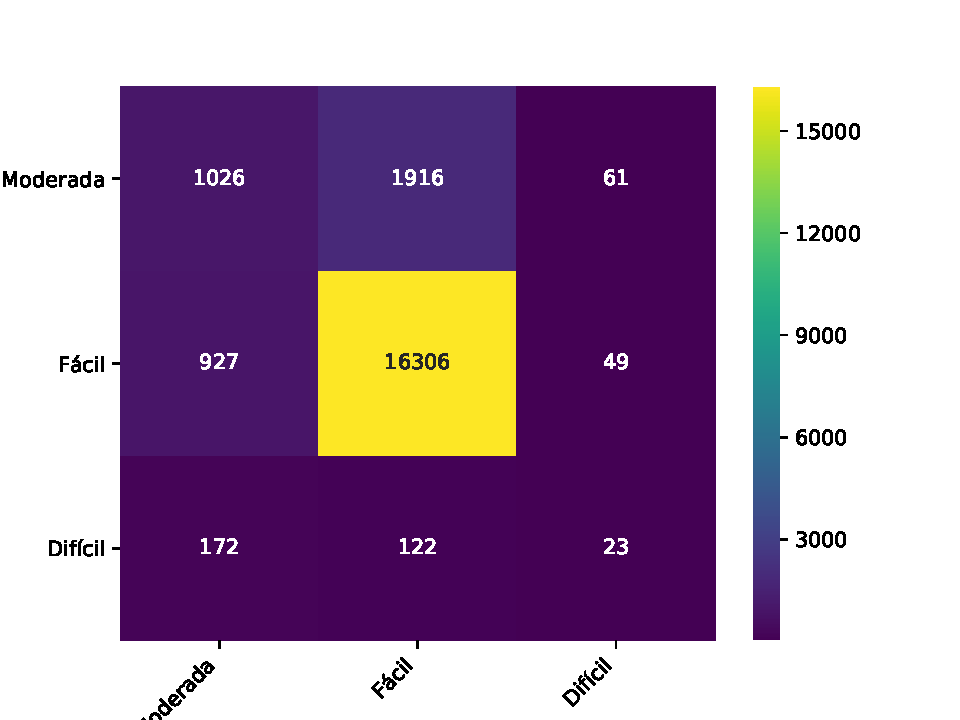
\includegraphics[width=\columnwidth]{cm}
	\caption{Matriz de confusión de una ejecución.}
	\label{fig:cm}
\end{figure}

\subsection{Importancia de las características}
Al usar random forest, la librería scikit-learn permite obtener la importancia de cada características en la predicción. Algunas de las más importantes son las relacionadas al historial del alumno (número medio de pistas, de fallos y de aciertos a la primera), aunque también hay algunos KCs aprendidos. En cualquier caso, la característica con más importancia tiene una importancia menor al 3\%, lo cual invita a pensar que estas no son muy útiles para este problema.

\section{Conclusiones}
La conclusión general que se saca es que el problema no se puede resolver correctamente con el planteamiento propuesto, sin embargo sí que se pueden obtener lecturas positivas y lecciones aprendidas del proceso.

Aunque los resultados han mostrado que el modelo no es muy bueno, sí que se puede ser algo útil a la hora de recomendar problemas de dificultad moderada, ya que, si se equivoca, el problema será fácil probablemente y no difícil, lo cual puede ser adecuado para el alumno.

Tal vez un modelo de red neuronal podría haber funcionado mejor porque combinaría de formas más específicas el aprendizaje con el KC necesario, sin embargo, esta técnica estaba prohibida.

Otro asunto a tener en cuenta es que los alumnos probablemente también recibieran clases sobre los temas y practicaran ejercicios fuera del tutor inteligente, así que el aprendizaje depende de más factores de los que se conocen. Además el modelo de aprendizaje temporal se ha ideado mediante suposiciones, así que si se hubiera tenido un modelo más adecuado podrían haberse mejorado los resultados.

Por último, merece la pena mencionar que, aunque los datos se hayan generado automáticamente por el log de un programa, estos tienen una cantidad de ruido nada desdeñable.

En definitiva: los resultados obtenidos no han sido muy buenos, sin embargo se han aprendido bastantes cosas en el proceso, sobre todo debido al haber abordado e problema desde un enfoque menos obvio que el propuesto por la competición.

\end{document}
